\documentclass{article}
\usepackage{amsfonts}
\usepackage{MnSymbol}
\usepackage{graphicx}
\title{Seminarium}
\begin{document}
    \section{Seminarie 2}
        \subsection{Problem 1}
            Hur många femsiffriga tal *utan nollor* finns det om\\
            \indent \textbf{a)} exakt en siffra skall vara udda?\\
            \indent \textbf{b)} minst tre siffror skall vara jämna, och ingen udda siffra får förekomma mer än en gång.
        
        \subsection{Problem 2}
            Låt $n\leq 3$ vara ett udda tal. $n$ stycken revolvermänstår i en öken. 
            Inga två revolvermän står på samma avstånd ifrån varandra. 
            Samtliga revolvermän drar sin revolver samtidigt och skjuter på den som står närmast. 
            Visa att minst en revolverman inte blir träffad.\\
        
        \subsection{Problem 3}
            Låt $n\in \mathbb{Z_{+}}$ och $K_{1,n}$ vara den fullständigt bipartita grafen med $1+n$ noder.\\
            \indent \textbf{a)} För vilka $n$ har $K_{1,n}$ en Eulerväg respektive en Eulercykel?\\
            \indent \textbf{b)} Om det finns en Eulercykel, 
            vad är det minsta antalet kanter man behöver ta bort och/eller lägga till för att det skall finnas en Eulercykel?
            Den resulterande grafen skall fortfarande vara sammanhängande.
        \clearpage
        \subsection{Lösningar}
            \subsubsection{Problem 1}
                \begin{tabbing}
                    \indent \textbf{a)}\hspace{5pt}\=\\
                    \>5 st udda siffror 1,3,5,7,9 och 4 st jämna siffror tillåtna 2,4,6,8\\
                    \>Vi har fem positioner vilket ger:\\
                    \>$5\cdot 5\cdot 4\cdot 4\cdot 4\cdot 4=6400$\\
                    \>där första 5 är val av position för det udda talet, andra 5 är val av udda tal, och fyrorna är val av jämna tal på resterande positioner\\\\
                \end{tabbing}

                \begin{tabbing}
                    \indent \textbf{b)}\hspace{5pt}\=\\
                    \>Vi har \underline{3 fall}:\\
                    \>\underline{Exakt 3 jämna}, dvs exakt två udda.\\
                    \>$\begin{pmatrix}5\\2\end{pmatrix}\cdot 5\cdot 4\cdot 4^{3}=12800$\\
                    \>$\begin{pmatrix}5\\2\end{pmatrix}$ är val av positioner för de udda talen, 
                    $5\cdot 4$ är val av udda tal (skall vara olika), 
                    $4^{3}$ är val av jämna tal\\\\
                    \>\underline{Exakt 4 jämna = exakt en udda}\\
                    \>Det är del a) - 6400 st\\\\
                    \>\underline{Exakt 5 jämna}\\
                    \>$4^{5}=1024$\\\\
                    \>\underline{Totalt} $12800+6400+1024=20224$
                \end{tabbing}
            
            \subsubsection{Problem 2}
                \underline{Induktion på n}, n udda, $\leq 3$, 3,5,7 etc\\
                \begin{tabbing}
                    \underline{Basfall n=3}\=\\
                    \>Alltid ett par med minsta avstånd mellan varandra.\\
                    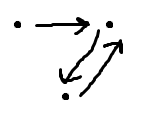
\includegraphics{img01.png}\\
                    \>De två skjuter på varandra, så den tredje personen blir inte träffad.
                \end{tabbing}
                \underline{Indutktionssteg}
                \begin{itemize}
                    \item Antag att, för n st revolvermän som skjuter på varandra, 
                        så blir en person inte träffad
                    \item Vill visa samma påstående fast med n+2 st revolvermän
                \end{itemize}
                Återigen, finns två st med minsta avstånd emellan varandra. De skjuter på varandra.\\
                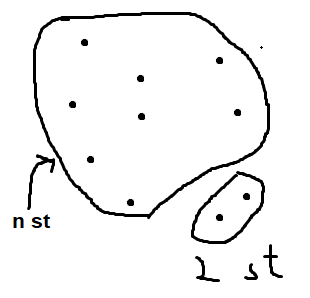
\includegraphics[scale=0.5]{img02.png}\\
                Vill applicera mitt induktionsantagande på dessa n st. Kan jag göra det?\\\\
                \underline{Kanske inte} Vissa av de n st kanske skjuter på de 2 andra.\\\\
                \underline{Fall 1:} Alla de n skjuter på varandra. 
                Då kan jag applicera induktionsantagandet.\\\\
                \underline{Fall 2:} Någon av de n skjuter på någon av de 2. 
                Hur många skott går mot gruppen med n st? Högst n-1 skott! 
                Då Enligt lådprincipen måste det finnas minst en person bland de n som inte blir träffad.
            
            \subsubsection{Problem 3}
                \begin{tabbing}
                    \indent \textbf{a)}\hspace{5pt}\=\\
                    \>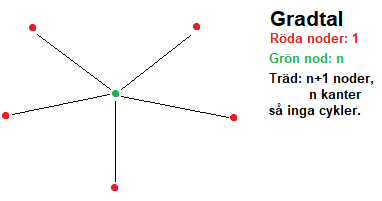
\includegraphics[scale=0.3]{img03.png}\\
                    \>Finns aldrig en Eulercykel (gradtalen är inte jämna)\\
                    \>\underline{Eulerväg?} ja, om det finns exakt två noder med udda gradtal. $\Rightarrow n\geq 2$.
                    Och då funkar det $k_{1,1}$, $k_{1,2}$
                \end{tabbing}
                \begin{tabbing}
                    \indent \textbf{a)}\hspace{5pt}\=\\
                    \>Behöver se till att alla gradtal är jämna och $\ge 0$\\
                    \>\underline{n jämnt:}\\\\
                    \>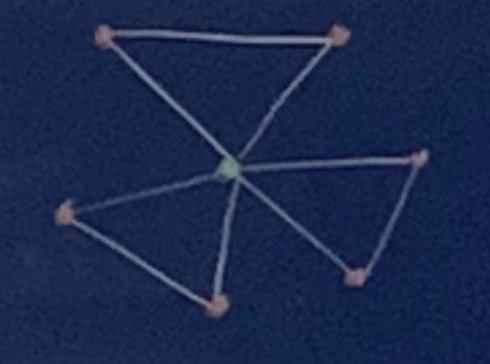
\includegraphics[scale=0.2]{img04.png}\\
                    \>lägger till $\frac{n}{2}$ kanter som i bilden. 
                    Alla röda kanternas gradtal 2, och den gröna har gradtal n.\\
                    \>\underline{n udda:}\\\\
                    \>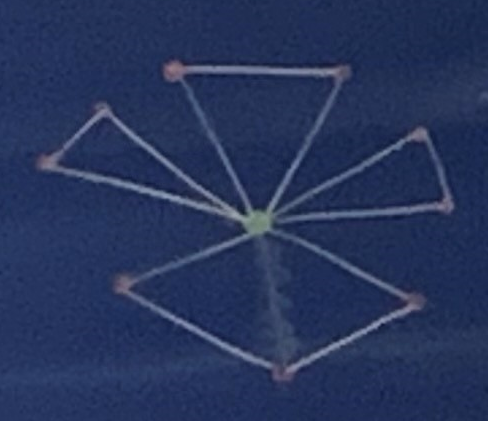
\includegraphics[scale=0.2]{img05.png}\\
                    \>lägger till $\frac{n+1}{2}$ --- bort 1 kant.
                \end{tabbing}
\end{document}